\documentclass[11pt,a4paper]{article}

\usepackage{fontspec}
\usepackage{geometry}
\usepackage{amsmath,amssymb,amsthm}
\usepackage{xcolor}
\usepackage{hyperref}
\usepackage{tikz}
\usetikzlibrary{calc}
\usepackage{float}

\geometry{margin=2.3cm}

\IfFontExistsTF{Noto Serif CJK SC}
  {\setmainfont{Noto Serif CJK SC}}
  {\setmainfont{Droid Sans Fallback}}
\IfFontExistsTF{Noto Sans CJK SC}
  {\setsansfont{Noto Sans CJK SC}}
  {\setsansfont{Droid Sans Fallback}}
\IfFontExistsTF{Noto Sans Mono CJK SC}
  {\setmonofont{Noto Sans Mono CJK SC}}
  {\setmonofont{Droid Sans Fallback}}

\XeTeXlinebreaklocale "zh"
\XeTeXlinebreakskip = 0pt plus 1pt minus 0.1pt
\linespread{1.15}

\hypersetup{
  colorlinks=true,
  linkcolor=blue,
  urlcolor=blue,
  citecolor=blue
}

\definecolor{lampA}{RGB}{198,43,42}
\definecolor{lampB}{RGB}{44,93,197}

\newtheorem{theorem}{定理}[section]
\newtheorem{lemma}[theorem]{引理}
\newtheorem{proposition}[theorem]{命题}
\theoremstyle{definition}
\newtheorem{definition}[theorem]{定义}

\renewcommand{\proofname}{证明}
\renewcommand{\abstractname}{摘要}
\renewcommand{\refname}{参考文献}

\title{\textbf{从一张图上读出的巴塞尔问题}\\[0.3em]
\large Wästlund 加倍构造中多出的一盏灯，与剩下只需计算的等比级数}
\author{YeXiaoRain\thanks{独立研究者，四川成都，中国，\texttt{yexiaorain@gmail.com}}}
\date{2026 年 11 月 20 日}

\begin{document}

\maketitle

\begin{abstract}
Wästlund 对巴塞尔问题的几何证明反复把圆翻倍，并把每一盏灯换成大圆上两盏等效灯，
观察点 $P$ 处的总亮度因此始终不变；极限下这张图交出的是正\emph{奇数}项的平方倒数和，
还要再补一次代数运算才能回到原级数。本文改动翻倍这一步：每轮在大圆上 $P$ 的正对面补上一盏灯。
正对面恰好是等效替换唯一产生不出来的位置，所以每轮恰好只缺一盏；补上的灯到 $P$ 的距离逐轮翻倍，
贡献排成等比级数，而极限直线上每个非零整数点都亮着灯。两侧亮度相等，
$\sum_{n\ge1}1/n^{2}=\pi^{2}/6$ 便直接从图上读出，不再绕道奇数项。
\end{abstract}

\begin{center}
\small
\textbf{MSC 2020：} 51M04（主）；40A05，11A25，01A50\\[0.3em]
\textbf{关键词：} 巴塞尔问题；几何证明；平方反比；反勾股定理；Wästlund 的构造
\end{center}

\section{引言}

巴塞尔问题要求算出所有正整数平方的倒数之和：
\begin{equation}
  S=\sum_{n=1}^{\infty}\frac{1}{n^{2}}
   =1+\frac{1}{2^{2}}+\frac{1}{3^{2}}+\frac{1}{4^{2}}+\cdots .
  \label{eq:basel}
\end{equation}
蒙戈利在 1644 年提出这个问题，欧拉在 1735 年算得它为 $\pi^{2}/6$。等式左边只由整数构成，
右边却是一个圆周率常数，于是自然会期待这一等式有一个几何读法。

这样的读法确实存在：Wästlund 在一篇短文里给出了只用欧几里得几何的证明 \cite{wastlund}，
后来的科普视频又让它流传到更广的读者中 \cite{threeblueonebrown}。整套构造只用到圆、
弦、直角和光的平方反比律：圆上的灯点看成点光源，两圆的公共切点 $P$ 看成观察点，
一项 $\frac{1}{d^{2}}$ 读成距离 $d$ 处那盏灯送到 $P$ 的亮度。圆每翻倍一次，
每盏灯就被大圆上两盏等效灯替换掉，$P$ 处的总亮度不变；极限下圆压成一条直线，
灯落在奇数整数处。

把构造归一化：周长为 $2$ 的圆上只有一盏灯，摆在 $P$ 的正对面，到 $P$ 的距离为 $\frac{2}{\pi}$。
这张图交出的是奇数项。

\begin{theorem}[Wästlund]\label{thm:wastlund}
在上述归一化下，几何构造给出
\begin{equation}
  \sum_{k=0}^{\infty}\frac{1}{(2k+1)^{2}}=\frac{\pi^{2}}{8}.
  \label{eq:odd-sum}
\end{equation}
\end{theorem}

要从定理 \ref{thm:wastlund} 得到 $S$，需要一句代数：偶数项之和是 $\frac14 S$，
于是 $\frac34 S=\frac{\pi^{2}}{8}$。这一句是整个论证里唯一的非几何步骤，
也正是本文要省掉的那一步。

\begin{theorem}[本文]\label{thm:direct}
把翻倍规则改成：每一轮先把灯按原样映射到大圆上，再在大圆上 $P$ 的正对面补一盏灯。
这样极限直线上每个非零整数点都亮着灯，它们送到 $P$ 的亮度等于各轮补上的灯的亮度，
\begin{equation}
  2S=\sum_{k=0}^{\infty}\frac{\pi^{2}}{4^{k+1}}=\frac{\pi^{2}}{3},
  \qquad\text{于是}\qquad
  S=\frac{\pi^{2}}{6}.
  \label{eq:direct}
\end{equation}
\end{theorem}

每轮只需补一盏灯，而且它永远落在同一个位置：正对面正是等效替换产生不出来的那一处，
因为它的原像得是 $P$ 本身的一盏灯。其余整数位置各被填上一次，不多不少。

等式 \eqref{eq:basel} 与 $\pi^{2}/6$ 早已有很多条到达路线：Kalman 的综述收了六条
\cite{kalman}，Matsuoka 给出一条初等的 \cite{matsuoka}；与下面这张图气质最接近的，
是 Dumont 那个启发式论证——Komornik 把它补严，并把 Gregory--Leibniz 级数与巴塞尔级数
系在一起 \cite{komornik}。就作者能查到的——论文与科普视频都查过——还没有哪张同类的图
能直接读出完整的级数本身：已有的几何讲法都停在某个子级数，再靠代数收尾。
本文要改动的都不是这几条路线，只针对 Wästlund 的这一支构造
\cite{wastlund}。

第 2 节复述 Wästlund 的证明；第 3 节给出改动与定理 \ref{thm:direct} 的证明，
那是本文唯一的新内容。

\section{Wästlund 的构造}\label{sec:wastlund}

\subsection{亮度与平方反比}

点光源向各方向均匀发光，观察者在垂直于入射方向的小面上接收。距离为 $r$ 时，
同样的光通量摊在面积为 $4\pi r^{2}$ 的球面上，所以单位面积的亮度为
\begin{equation}
  B(r)=\frac{L}{4\pi r^{2}}\propto\frac{1}{r^{2}}.
  \label{eq:inverse-square}
\end{equation}
距离翻倍，亮度只剩四分之一。全文都把灯到观察点 $P$ 的距离代入这一式子，
因此 $\sum\frac{1}{d^{2}}$ 读起来就是 $P$ 处的总亮度。

\begin{definition}[灯、亮度与等效]\label{def:lamps}
平面上取定一点 $P$，称为\emph{观察点}。一盏\emph{灯}是某个 $Q\neq P$ 处的点光源，
它在 $P$ 处的\emph{亮度}就是数量 $\frac{1}{PQ^{2}}$；有限盏或可数盏灯的\emph{总亮度}
是各自亮度之和。若 $\frac{1}{PS_{1}^{2}}+\frac{1}{PS_{2}^{2}}=\frac{1}{PR^{2}}$，
就说两盏灯 $S_{1},S_{2}$（在 $P$ 处）\emph{等效于}一盏灯 $R$。
若过 $P$ 的圆以 $O$ 为圆心，则该圆上与 $P$ 直径相对的点称为 $P$ 的\emph{正对面}。
\end{definition}

有了这套说法，把一盏灯换成两盏等效灯就不改变总亮度，
需要核验的只剩反勾股恒等式，即引理 \ref{lem:inverse-pythagoras}。

\subsection{反勾股定理}

\begin{lemma}[反勾股]\label{lem:inverse-pythagoras}
设直角三角形的两条直角边为 $a,b$，斜边为 $c$，斜边上的高为 $h$，则
\begin{equation}
  \frac{1}{h^{2}}
  =\frac{c^{2}}{a^{2}b^{2}}
  =\frac{a^{2}+b^{2}}{a^{2}b^{2}}
  =\frac{1}{a^{2}}+\frac{1}{b^{2}}.
  \label{eq:inverse-pythagoras}
\end{equation}
\end{lemma}

\begin{proof}
两种面积表达式给出 $ab=ch$，于是 $c^{2}h^{2}=a^{2}b^{2}$；再代入 $c^{2}=a^{2}+b^{2}$
即得式 \eqref{eq:inverse-pythagoras}。
\end{proof}

\begin{figure}[htbp]
\centering
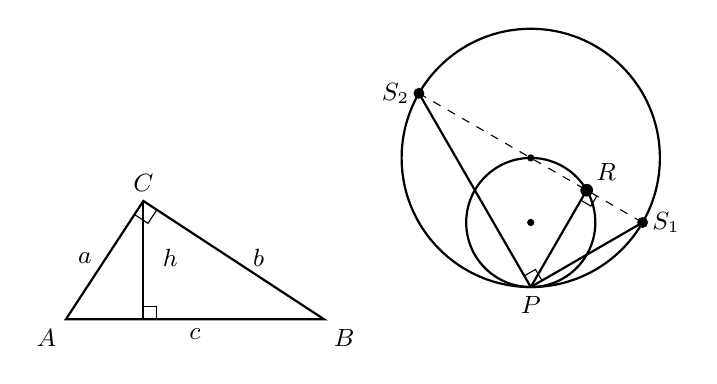
\begin{tikzpicture}[scale=0.82, every node/.style={font=\small}]
  \begin{scope}
    \coordinate (A) at (0,0);
    \coordinate (B) at (4,0);
    \coordinate (C) at (1.2,1.833);
    \coordinate (H) at (1.2,0);
    \draw[thick] (A)--(B)--(C)--cycle;
    \draw[thick] (C)--(H);
    \draw (1.4,0)--(1.4,0.2)--(1.2,0.2);
    \draw (1.063,1.624)--(1.272,1.487)--(1.409,1.696);
    \node[left] at (0.55,0.95) {$a$};
    \node[right] at (2.75,0.95) {$b$};
    \node[right] at (1.35,0.95) {$h$};
    \node[below] at (2,0) {$c$};
    \node[below left] at (A) {$A$};
    \node[below right] at (B) {$B$};
    \node[above] at (C) {$C$};
  \end{scope}

  \begin{scope}[shift={(7.2,0.5)}]
    \coordinate (P) at (0,0);
    \coordinate (O1) at (0,1);
    \coordinate (O2) at (0,2);
    \draw[thick] (O1) circle (1);
    \draw[thick] (O2) circle (2);
    \coordinate (R) at (0.866,1.5);
    \coordinate (S1) at (1.732,1);
    \coordinate (S2) at (-1.732,3);
    \draw[dashed] (S2)--(S1);
    \draw[thick] (P)--(R);
    \draw[thick] (P)--(S1);
    \draw[thick] (P)--(S2);
    \fill (R) circle (2.8pt);
    \fill (S1) circle (2.4pt);
    \fill (S2) circle (2.4pt);
    \fill (O1) circle (1.6pt);
    \fill (O2) circle (1.6pt);
    \draw (0.776,1.344)--(0.932,1.254)--(1.022,1.410);
    \draw (0.173,0.1)--(0.073,0.273)--(-0.1,0.173);
    \node[above right] at (R) {$R$};
    \node[right] at (S1) {$S_1$};
    \node[left] at (S2) {$S_2$};
    \node[below] at (P) {$P$};
  \end{scope}
\end{tikzpicture}
\caption{左：反勾股定理。右：引理 \ref{lem:replacement} 的替换。}
\label{fig:circle-replacement}
\end{figure}

\subsection{一盏灯换成两盏等效灯}

\begin{lemma}[替换]\label{lem:replacement}
设圆 $C_{1},C_{2}$ 的半径分别为 $r_{1}$ 与 $r_{2}=2r_{1}$，相切于观察点 $P$，
$R$ 是 $C_{1}$ 上的一盏灯。过 $R$ 作 $PR$ 的垂线，交 $C_{2}$ 于 $S_{1},S_{2}$，则
\begin{equation}
  \underbrace{\frac{1}{PR^{2}}}_{C_{1}\text{ 上一盏灯}}
  \;=\;
  \underbrace{\frac{1}{PS_{1}^{2}}+\frac{1}{PS_{2}^{2}}}_{C_{2}\text{ 上两盏灯}}.
  \label{eq:replacement}
\end{equation}
\end{lemma}

\begin{proof}
$C_{1}$ 上与 $P$ 直径相对的点在连心线上，到 $P$ 的距离是 $2r_{1}=r_{2}$，
所以它正是 $C_{2}$ 的圆心 $O_{2}$。因为 $PO_{2}$ 是 $C_{1}$ 的直径，角 $PRO_{2}$ 是直角：
过 $R$ 垂直于 $PR$ 的直线就是 $RO_{2}$，它在 $C_{2}$ 上截出的是一段直径的两个端点。
于是 $S_{1}S_{2}$ 是 $C_{2}$ 的直径，而 $P$ 在 $C_{2}$ 上，所以角 $S_{1}PS_{2}$ 是直角，
$PR$ 恰是它斜边上的高。把引理 \ref{lem:inverse-pythagoras} 用于三角形 $PS_{1}S_{2}$，
得到的正是式 \eqref{eq:replacement}。
\end{proof}

换句话说，小圆上的一盏灯可以换成大圆上的两盏灯，而 $P$ 处的亮度不变。

\subsection{翻倍：$N$ 等分点换成 $2N$ 等分点}

\begin{lemma}[翻倍]\label{lem:doubling}
在 $C_{1}$ 的 $N$ 个等分点各放一盏灯，逐盏按引理 \ref{lem:replacement} 换成 $C_{2}$ 上的像。
这些像正是与它们\emph{对应的} $C_{2}$ 的 $2N$ 等分点，且 $P$ 处的总亮度不变。
\end{lemma}

\begin{proof}
一盏灯 $R$ 的像是一对点，即过 $R$ 与 $O_{2}$ 的直径的两端，于是整幅图就是一束过 $O_{2}$ 的射线。
因为 $O_{2}$ 在 $C_{1}$ 上，相邻射线之间的角是 $C_{1}$ 上等弦所对的圆周角，两两相等；
同一批角又是 $C_{2}$ 的圆心角，所以射线与 $C_{2}$ 交出的 $2N$ 个点把 $C_{2}$ 等分。
亮度逐盏守恒，由引理 \ref{lem:replacement} 给出。
\end{proof}

「对应的」三个字要紧：这 $2N$ 个点是 $N$ 盏灯逐盏产生的，
任意取一组 $2N$ 等分点并不保持亮度。

\begin{figure}[htbp]
\centering
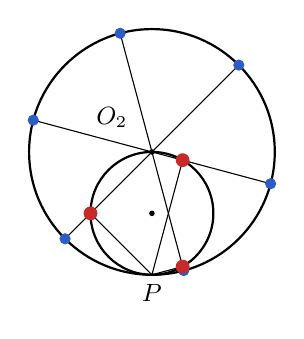
\begin{tikzpicture}[scale=0.78, every node/.style={font=\small}]
  \coordinate (P) at (0,0);
  \coordinate (O1) at (0,1);
  \coordinate (O2) at (0,2);
  \draw[thick] (O1) circle (1);
  \draw[thick] (O2) circle (2);
  \coordinate (R1) at (0.5,1.866);
  \coordinate (R2) at (0.5,0.134);
  \coordinate (R3) at (-1,1);
  \foreach \a [evaluate=\a as \c using {\a+180}] in {45,105,165}
    \draw[thin] ($(O2)+(\a:2)$)--($(O2)+(\c:2)$);
  \draw[thin] (P)--(R1);
  \draw[thin] (P)--(R2);
  \draw[thin] (P)--(R3);
  \foreach \a in {45,105,165,225,285,345}
    \fill[lampB] ($(O2)+(\a:2)$) circle (2.6pt);
  \fill[lampA] (R1) circle (3.2pt);
  \fill[lampA] (R2) circle (3.2pt);
  \fill[lampA] (R3) circle (3.2pt);
  \fill (O1) circle (1.3pt);
  \fill (O2) circle (1.3pt);
  \node[above left] at ($(O2)+(-0.24,0.24)$) {$O_2$};
  \node[below] at (P) {$P$};
\end{tikzpicture}
\caption{小圆的 $3$ 等分点换成大圆上对应的 $6$ 等分点。}
\label{fig:doubling}
\end{figure}

\subsection{极限：圆变成直线}

取周长为 $2$ 的圆，即半径 $R_{0}=\frac{1}{\pi}$，唯一的灯摆在 $P$ 的正对面。
它到 $P$ 的距离是 $\frac{2}{\pi}$，所以 $P$ 处的总亮度为
\begin{equation}
  \frac{1}{d^{2}}=\frac{1}{(2/\pi)^{2}}=\frac{\pi^{2}}{4}.
  \label{eq:first-lamp}
\end{equation}

\begin{figure}[H]
\centering
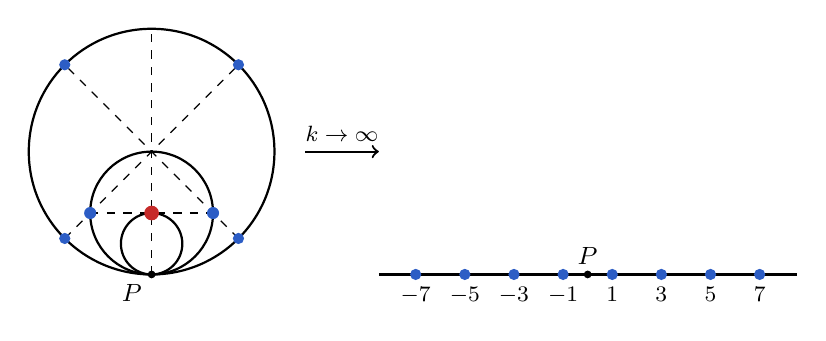
\begin{tikzpicture}[scale=0.78, every node/.style={font=\small}]
  \draw[dashed] (0,0)--(0,4);
  \draw[thick] (0,0.5) circle (0.5);
  \draw[thick] (0,1) circle (1);
  \draw[thick] (0,2) circle (2);
  \draw[thin,dashed] (-1,1)--(1,1);
  \draw[thin,dashed] (1.414,0.586)--(-1.414,3.414);
  \draw[thin,dashed] (-1.414,0.586)--(1.414,3.414);
  \fill[lampB] (1.414,0.586) circle (2.6pt);
  \fill[lampB] (-1.414,0.586) circle (2.6pt);
  \fill[lampB] (1.414,3.414) circle (2.6pt);
  \fill[lampB] (-1.414,3.414) circle (2.6pt);
  \fill[lampB] (1,1) circle (2.8pt);
  \fill[lampB] (-1,1) circle (2.8pt);
  \fill[lampA] (0,1) circle (3.4pt);
  \fill (0,0) circle (1.8pt);
  \node[below left] at (0,0) {$P$};
  \draw[->,thick] (2.5,2)--(3.7,2);
  \node[above,font=\footnotesize] at (3.1,2) {$k\to\infty$};
  \begin{scope}[shift={(7.1,0)}]
    \draw[thick] (-3.4,0)--(3.4,0);
    \fill (0,0) circle (1.8pt);
    \node[above] at (0,0) {$P$};
    \foreach \x/\lab in {-2.8/-7,-2.0/-5,-1.2/-3,-0.4/-1,0.4/1,1.2/3,2.0/5,2.8/7} {
      \fill[lampB] (\x,0) circle (2.6pt);
      \node[below,font=\footnotesize] at (\x,-0.05) {$\lab$};
    }
  \end{scope}
\end{tikzpicture}
\caption{半径逐轮翻倍，极限下圆压成过 $P$ 的直线。}
\label{fig:doubling-limit}
\end{figure}

每次翻倍都保持这一总亮度，翻倍 $k$ 次之后，周长 $2^{k+1}$ 的圆上的灯落在离 $P$
弧长 $1,3,5,\dots$ 处。当 $k\to\infty$ 时圆趋于它在 $P$ 的切线，弦长趋于弧长，
灯就落在直线上的 $\pm1,\pm3,\pm5,\dots$（图 \ref{fig:doubling-limit}），于是
\begin{equation}
  2\left(1+\frac{1}{3^{2}}+\frac{1}{5^{2}}+\cdots\right)=\frac{\pi^{2}}{4},
  \label{eq:odd-limit}
\end{equation}
两边除以 $2$ 就证明了定理 \ref{thm:wastlund}。

\subsection{回到巴塞尔问题}

式 \eqref{eq:basel} 的偶数项是整体级数的 $\frac14$，配上式 \eqref{eq:odd-sum} 就有
\begin{equation}
  \resizebox{\textwidth}{!}{$
  \begin{array}{r*{21}{c}r}
    &1&&&+&\frac{1}{3^{2}}&&&+&\frac{1}{5^{2}}&&&+&\frac{1}{7^{2}}&&&+&\frac{1}{9^{2}}
    &&&+&\cdots&=\frac{\pi^{2}}{8}\\[14pt]
    S=&1&+&\frac{1}{2^{2}}&+&\frac{1}{3^{2}}&+&\frac{1}{4^{2}}&+&\frac{1}{5^{2}}
    &+&\frac{1}{6^{2}}&+&\frac{1}{7^{2}}&+&\frac{1}{8^{2}}&+&\frac{1}{9^{2}}
    &+&\frac{1}{10^{2}}&+&\cdots&\\[20pt]
    \frac{1}{4}S=&&&\frac{1}{2^{2}}&&&+&\frac{1}{4^{2}}&&&+&\frac{1}{6^{2}}
    &&&+&\frac{1}{8^{2}}&&&+&\frac{1}{10^{2}}&+&\cdots&
  \end{array}$}
  \label{eq:odd-even}
\end{equation}
于是 $S=\frac{\pi^{2}}{8}\cdot\frac{1}{1-\frac14}=\frac{\pi^{2}}{6}$。最后这一段计算，
正是下面的定理 \ref{thm:direct} 要避开的代数步骤：式 \eqref{eq:odd-even} 把 $S$ 换成了
$\frac34 S$，图上的信息也就跟着换成了它的奇数项子级数。

\section{多走一步：每轮只补一盏灯}\label{sec:one-more-step}

第 2 节交出的只有奇数项。我们把翻倍规则改动一处：每一轮先把小圆上的灯按引理
\ref{lem:replacement} 映射到大圆上，再在大圆上 $P$ 的正对面补一盏灯。

\begin{lemma}[缺位]\label{lem:missing}
设第 $k$ 轮圆的周长为 $C=2^{k+1}$，半径 $\frac{2^{k}}{\pi}$，灯落在从 $P$ 量的
弧距 $s=1,2,\dots,C-1$ 处。按引理 \ref{lem:doubling} 替换之后，大圆上的灯占满整数弧距
$1,\dots,2C-1$ 中除 $s=C$ 以外的每一处，而 $s=C$ 正是 $P$ 的正对面；第 $k$ 轮圆上没有任何灯
能被映射到那里。
\end{lemma}

\begin{proof}
第 $k$ 轮圆上弧距 $s$ 的灯，被换成大圆上过它的直径的两端，即弧距 $s$ 与 $s+C$；
于是 $1,\dots,2C-1$ 中除 $C$ 之外每处恰好被填一次。弧距 $C$ 那点位于过 $P$ 的直径另一端，
也就是连心线；这条线在第 $k$ 轮圆上的另一个点是 $P$ 本身，那里没有灯。所以正对面没有原像。
\end{proof}

\begin{proposition}[补上的灯的亮度]\label{prop:added}
第 $k$ 轮补上的那盏灯到 $P$ 的距离是 $\frac{2^{k+1}}{\pi}$，按式 \eqref{eq:inverse-square}
贡献亮度 $\frac{\pi^{2}}{4^{k+1}}$；各轮补的灯合起来是
\begin{equation}
  B=\sum_{k=0}^{\infty}\frac{\pi^{2}}{4^{k+1}}
   =\frac{\pi^{2}}{4}\cdot\frac{1}{1-\frac14}
   =\frac{\pi^{2}}{3}.
  \label{eq:supplement-brightness}
\end{equation}
\end{proposition}

\begin{proof}
$P$ 到正对面的距离就是第 $k$ 轮圆的直径 $\frac{2^{k+1}}{\pi}$；剩下的和是公比 $\frac14$
的等比级数。
\end{proof}

\begin{proof}[定理 \ref{thm:direct} 的证明]
半径趋于无穷时，圆压成过 $P$ 的切线，弦长趋于弧长，而由引理 \ref{lem:missing}
每个整数位置都被点亮：极限直线上全体非零整数处都有灯，到 $P$ 的距离依次是
$1,2,3,\dots$（图 \ref{fig:onepic}）。它们送到 $P$ 的亮度是
$\sum_{n\neq0}\frac{1}{n^{2}}=2S$。由引理 \ref{lem:replacement}，替换不改变 $P$ 处的亮度，
所以这一总亮度就等于各轮不得不补上的那些灯的亮度 \eqref{eq:supplement-brightness}，
即 $2S=\frac{\pi^{2}}{3}$，亦即 $S=\frac{\pi^{2}}{6}$。
\end{proof}

\begin{figure}[H]
\centering
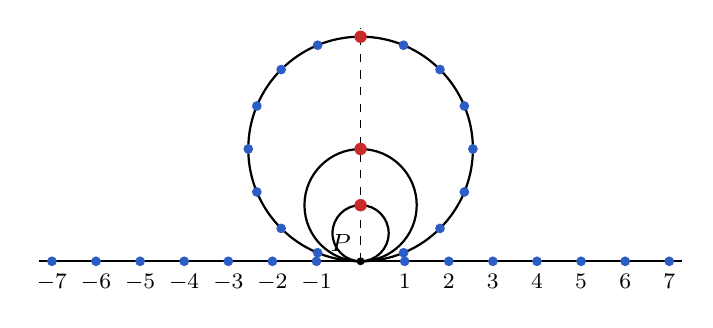
\begin{tikzpicture}[scale=0.8, every node/.style={font=\small}]
  \coordinate (P) at (0,0);
  % 圆与直线共用一个尺度：每单位弧长（每单位距离）取 0.7，
  % 于是周长 $2^{k+1}$ 的圆半径是 $0.7\cdot 2^k/\pi$。
  \draw[thick] (0,0.446) circle (0.446);
  \draw[thick] (0,0.891) circle (0.891);
  \draw[thick] (0,1.783) circle (1.783);
  \draw[thin,dashed] (0,0)--(0,3.7);
  \foreach \s [evaluate=\s as \ang using {180*\s/8-90}] in {1,2,3,4,5,6,7,9,10,11,12,13,14,15}
    \fill[lampB] (0,1.783) + (\ang:1.783) circle (2.2pt);
  \fill[lampA] (0,0.891) circle (2.8pt);
  \fill[lampA] (0,1.783) circle (2.8pt);
  \fill[lampA] (0,3.565) circle (2.8pt);
  \draw[thick] (-5.1,0)--(5.1,0);
  \foreach \x/\lab in {-4.9/-7,-4.2/-6,-3.5/-5,-2.8/-4,-2.1/-3,-1.4/-2,-0.7/-1,0.7/1,1.4/2,2.1/3,2.8/4,3.5/5,4.2/6,4.9/7} {
    \fill[lampB] (\x,0) circle (2.2pt);
    \node[below,font=\footnotesize] at (\x,-0.05) {$\lab$};
  }
  \fill (P) circle (1.8pt);
  \node[above left] at (P) {$P$};
\end{tikzpicture}
\caption{一张图讲完整个证明：翻倍的圆与极限直线按同一尺度重合于 $P$，红色是每轮补上的灯。}
\label{fig:onepic}
\end{figure}

与第 2.4--2.5 节的区别只有一点：那里每轮都是纯粹的等效替换，总亮度守恒，
极限下读出的是奇数项；这里亮度逐轮累加，代价是每轮补一盏灯，换来的则是
式 \eqref{eq:basel} 本身出现在图上，而不是它的某个子级数。
式 \eqref{eq:supplement-brightness} 的每一项都能在图上指着一盏灯说出来，
这正是式 \eqref{eq:odd-even} 那次代数做不到的。

\section*{致谢}

几何构造出自 Johan Wästlund 的短文，本文只是在他的图上多走了一步；
3Blue1Brown 的视频是让这一构造直观起来的科普版本，本文的整理也受益于它。

{\small
\begin{thebibliography}{9}

\bibitem{wastlund}
J. Wästlund, \emph{Summing inverse squares by euclidean geometry},
Chalmers University of Technology, 哥德堡，2010 年 12 月 8 日，未刊文稿。
\url{https://www.math.chalmers.se/~wastlund/Cosmic.pdf}

\bibitem{threeblueonebrown}
3Blue1Brown, \emph{Why is pi here? And why is it squared? A geometric answer to the Basel problem},
YouTube，2018 年 3 月 3 日。
\url{https://www.youtube.com/watch?v=d-o3eB9sfls}

\bibitem{kalman}
D. Kalman, \emph{Six ways to sum a series}, College Mathematics Journal 24 卷 5 期，402--421 页，1993 年。

\bibitem{matsuoka}
Y. Matsuoka, \emph{An elementary proof of the formula $\sum 1/k^{2}=\pi^{2}/6$},
American Mathematical Monthly 68 卷 5 期，1961 年。

\bibitem{komornik}
V. Komornik, \emph{A ``luminous'' solution to the Basel problem},
Mathematics Magazine 95 卷 4 期，333--337 页，2022 年。

\end{thebibliography}}


\end{document}
